\section{Stochastic stability near coexistence}\label{sec:noise}
Following Sections 3.3--3.4 of \citet{haque11}, we consider white and colored perturbations around a positive equilibrium. We work with local linear models and specify the noise separately from the deterministic system. Write \(u=((x-x^*)/k,(y-y^*)/\beta)^\top\), and let \(J\) be the Jacobian in these scaled density coordinates, with time \(t\) unchanged. Assume \(J\) is Hurwitz, meaning that both eigenvalues have negative real part.

\subsection{Independent multiplicative white noise}
Let \(W_1,W_2\) be independent standard Wiener processes. With coordinate projections \(P_i\) and noise intensities \(\sigma_i\), consider the It\^o system
\[
 \dd u=Ju\,\dd t+\sum_{i=1}^2 B_i u\,\dd W_i,\qquad B_i=\sigma_iP_i.
\]
Let \(P=P^\top>0\) solve \(J^\top P+PJ=-I\). It\^o's formula gives
\[
 \frac{\dd}{\dd t}\mathbb E[u^\top Pu]
 =-\mathbb E\!\left[u^\top
       \left(I-\textstyle\sum_i B_i^\top PB_i\right)u\right].
\]
Thus \(I-\sum_i B_i^\top PB_i>0\) is sufficient for exponential mean-square stability. If its smallest eigenvalue is \(\epsilon>0\), the right side is at most \(-\epsilon\,\mathbb E[u^\top Pu]/\lambda_{\max}(P)\). The eigenvalue bounds on \(P\) then give exponential decay of \(\mathbb E\|u(t)\|^2\). The plotted moments are obtained from the exact matrix equation \(\dot C_u=JC_u+C_uJ^\top+\sum_iB_iC_uB_i^\top\), where \(C_u=\mathbb E[uu^\top]\).

\subsection{A common Ornstein--Uhlenbeck fluctuation}
To obtain an explicit colored-noise bound, let a common scalar fluctuation \(\xi(t)\) modulate both coordinates, so \(\dot u=(J+\xi I)u\). Take \(\xi\) to be a stationary, mean-zero Ornstein--Uhlenbeck process with variance \(q>0\) and covariance \(q e^{-\theta |t-s|}\), \(\theta>0\). For fixed \(u(0)\), the matrices commute and hence
\[
 u(t)=e^{Jt}u(0)\exp\!\left(\int_0^t \xi(s)\,\dd s\right),\qquad
 V_\xi(t)=2q\left[\frac{t}{\theta}-\frac{1-e^{-\theta t}}{\theta^2}\right],
\]
where \(V_\xi(t)\) is the variance of the integral. The Gaussian exponential moment gives \(\mathbb E\|u(t)\|^2=e^{2V_\xi(t)}\|e^{Jt}u(0)\|^2\). If \(2q/\theta<-\max\Real\operatorname{spec} J\), choose \(\gamma\) strictly between these values. Since \(\|e^{Jt}\|\le K_\gamma e^{-\gamma t}\), the second moment decays exponentially. This condition applies to the stated common modulation of the local linear system.

\subsection{A numerical check}
At \((r,k,\alpha,m,\beta,e,d)=(1,10,0.2,1.76,1,1/6,0.88)\), the coexistence equilibrium is \((6,1)\) and the largest real part of the Jacobian eigenvalues is \(-0.64\). For \((\sigma_1,\sigma_2)=(0.35,0.45)\), the minimum eigenvalue in the white-noise dissipation test is \(0.803895\). For \((q,\theta)=(0.12,1.2)\), the colored-noise threshold gives \(2q/\theta=0.2<0.64\). The white-noise moment calculation agrees with a separate integration of the moment equation to \(5.8\times10^{-15}\) in absolute error. Numerical quadrature of the colored-noise covariance agrees with the closed variance at the five checked times to \(2.3\times10^{-16}\).

\begin{figure}[!htbp]\centering
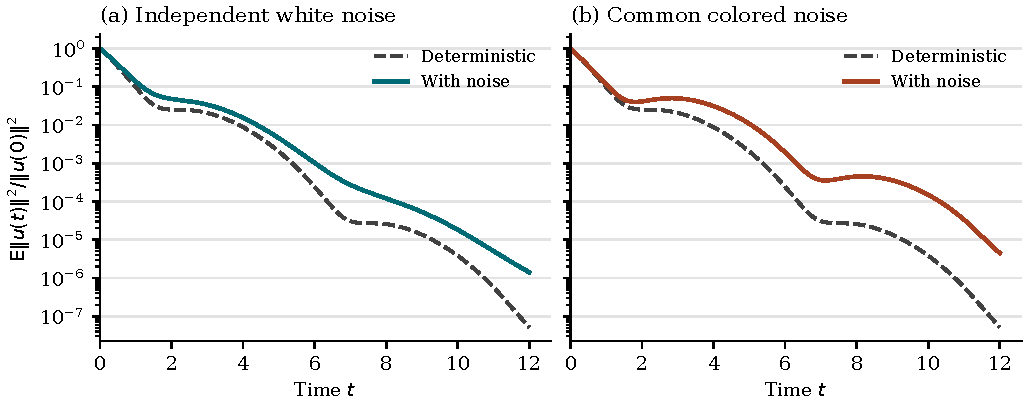
\includegraphics[width=\linewidth]{figures/stoch_moments.pdf}
\caption{Second moments for the two local perturbation models, both starting at \(u(0)=(0.01,-0.02)^\top\). A logarithmic axis shows the decay compared with the deterministic displacement. The curves come from the moment equations and the integrated Gaussian variance. Generated by \protect\path{code/stochastic_stability.py}.}\label{fig:noise}
\end{figure}
